\documentclass[]{article}
\usepackage{lmodern}
\usepackage{amssymb,amsmath}
\usepackage{ifxetex,ifluatex}
\usepackage{bm}
\usepackage{soul}
\usepackage[color=yellow]{todonotes}
\usepackage{fixltx2e} % provides \textsubscript
\ifnum 0\ifxetex 1\fi\ifluatex 1\fi=0 % if pdftex
  \usepackage[T1]{fontenc}
  \usepackage[utf8]{inputenc}
\else % if luatex or xelatex
  \ifxetex
    \usepackage{mathspec}
  \else
    \usepackage{fontspec}
  \fi
  \defaultfontfeatures{Ligatures=TeX,Scale=MatchLowercase}
\fi
% use upquote if available, for straight quotes in verbatim environments
\IfFileExists{upquote.sty}{\usepackage{upquote}}{}
% use microtype if available
\IfFileExists{microtype.sty}{%
\usepackage{microtype}
\UseMicrotypeSet[protrusion]{basicmath} % disable protrusion for tt fonts
}{}
\usepackage[margin=1in]{geometry}
\usepackage{hyperref}
\hypersetup{unicode=true,
            pdftitle={6 Extending the ARMA model: Seasonality and trend},
            pdfauthor={Edward Ionides},
            pdfborder={0 0 0},
            breaklinks=true}
\urlstyle{same}  % don't use monospace font for urls
\usepackage{color}
\usepackage{fancyvrb}
\newcommand{\VerbBar}{|}
\newcommand{\DEF}{\overset{\text{def}}{=}}
\newcommand{\PP}{\mathbb{P}}
\newcommand{\RR}{\mathbb{R}}
\newcommand{\ZZ}{\mathbb{Z}}
\newcommand{\EE}{\mathbb{E}}
\newcommand{\VERB}{\Verb[commandchars=\\\{\}]}
\DefineVerbatimEnvironment{Highlighting}{Verbatim}{commandchars=\\\{\}}
% Add ',fontsize=\small' for more characters per line
\usepackage{framed}
\definecolor{shadecolor}{RGB}{248,248,248}
\newenvironment{Shaded}{\begin{snugshade}}{\end{snugshade}}
\newcommand{\KeywordTok}[1]{\textcolor[rgb]{0.13,0.29,0.53}{\textbf{#1}}}
\newcommand{\DataTypeTok}[1]{\textcolor[rgb]{0.13,0.29,0.53}{#1}}
\newcommand{\DecValTok}[1]{\textcolor[rgb]{0.00,0.00,0.81}{#1}}
\newcommand{\BaseNTok}[1]{\textcolor[rgb]{0.00,0.00,0.81}{#1}}
\newcommand{\FloatTok}[1]{\textcolor[rgb]{0.00,0.00,0.81}{#1}}
\newcommand{\ConstantTok}[1]{\textcolor[rgb]{0.00,0.00,0.00}{#1}}
\newcommand{\CharTok}[1]{\textcolor[rgb]{0.31,0.60,0.02}{#1}}
\newcommand{\SpecialCharTok}[1]{\textcolor[rgb]{0.00,0.00,0.00}{#1}}
\newcommand{\StringTok}[1]{\textcolor[rgb]{0.31,0.60,0.02}{#1}}
\newcommand{\VerbatimStringTok}[1]{\textcolor[rgb]{0.31,0.60,0.02}{#1}}
\newcommand{\SpecialStringTok}[1]{\textcolor[rgb]{0.31,0.60,0.02}{#1}}
\newcommand{\ImportTok}[1]{#1}
\newcommand{\CommentTok}[1]{\textcolor[rgb]{0.56,0.35,0.01}{\textit{#1}}}
\newcommand{\DocumentationTok}[1]{\textcolor[rgb]{0.56,0.35,0.01}{\textbf{\textit{#1}}}}
\newcommand{\AnnotationTok}[1]{\textcolor[rgb]{0.56,0.35,0.01}{\textbf{\textit{#1}}}}
\newcommand{\CommentVarTok}[1]{\textcolor[rgb]{0.56,0.35,0.01}{\textbf{\textit{#1}}}}
\newcommand{\OtherTok}[1]{\textcolor[rgb]{0.56,0.35,0.01}{#1}}
\newcommand{\FunctionTok}[1]{\textcolor[rgb]{0.00,0.00,0.00}{#1}}
\newcommand{\VariableTok}[1]{\textcolor[rgb]{0.00,0.00,0.00}{#1}}
\newcommand{\ControlFlowTok}[1]{\textcolor[rgb]{0.13,0.29,0.53}{\textbf{#1}}}
\newcommand{\OperatorTok}[1]{\textcolor[rgb]{0.81,0.36,0.00}{\textbf{#1}}}
\newcommand{\BuiltInTok}[1]{#1}
\newcommand{\ExtensionTok}[1]{#1}
\newcommand{\PreprocessorTok}[1]{\textcolor[rgb]{0.56,0.35,0.01}{\textit{#1}}}
\newcommand{\AttributeTok}[1]{\textcolor[rgb]{0.77,0.63,0.00}{#1}}
\newcommand{\RegionMarkerTok}[1]{#1}
\newcommand{\InformationTok}[1]{\textcolor[rgb]{0.56,0.35,0.01}{\textbf{\textit{#1}}}}
\newcommand{\WarningTok}[1]{\textcolor[rgb]{0.56,0.35,0.01}{\textbf{\textit{#1}}}}
\newcommand{\AlertTok}[1]{\textcolor[rgb]{0.94,0.16,0.16}{#1}}
\newcommand{\ErrorTok}[1]{\textcolor[rgb]{0.64,0.00,0.00}{\textbf{#1}}}
\newcommand{\NormalTok}[1]{#1}
\usepackage{graphicx,grffile}
\makeatletter
\def\maxwidth{\ifdim\Gin@nat@width>\linewidth\linewidth\else\Gin@nat@width\fi}
\def\maxheight{\ifdim\Gin@nat@height>\textheight\textheight\else\Gin@nat@height\fi}
\makeatother
% Scale images if necessary, so that they will not overflow the page
% margins by default, and it is still possible to overwrite the defaults
% using explicit options in \includegraphics[width, height, ...]{}
\setkeys{Gin}{width=\maxwidth,height=\maxheight,keepaspectratio}
\IfFileExists{parskip.sty}{%
\usepackage{parskip}
}{% else
\setlength{\parindent}{0pt}
\setlength{\parskip}{6pt plus 2pt minus 1pt}
}
\setlength{\emergencystretch}{3em}  % prevent overfull lines
\providecommand{\tightlist}{%
  \setlength{\itemsep}{0pt}\setlength{\parskip}{0pt}}
%\setcounter{secnumdepth}{0}
\setcounter{section}{6}
% Redefines (sub)paragraphs to behave more like sections
\ifx\paragraph\undefined\else
\let\oldparagraph\paragraph
\renewcommand{\paragraph}[1]{\oldparagraph{#1}\mbox{}}
\fi
\ifx\subparagraph\undefined\else
\let\oldsubparagraph\subparagraph
\renewcommand{\subparagraph}[1]{\oldsubparagraph{#1}\mbox{}}
\fi

%%% Use protect on footnotes to avoid problems with footnotes in titles
\let\rmarkdownfootnote\footnote%
\def\footnote{\protect\rmarkdownfootnote}

%%% Change title format to be more compact
\usepackage{titling}

% Create subtitle command for use in maketitle
\newcommand{\subtitle}[1]{
  \posttitle{
    \begin{center}\large#1\end{center}
    }
}

\setlength{\droptitle}{-2em}
  \title{6. Extending the ARMA model: Seasonality and trend}
  \pretitle{\vspace{\droptitle}\centering\huge}
  \posttitle{\par}
  \author{Edward Ionides}
  \preauthor{\centering\large\emph}
  \postauthor{\par}
  \predate{\centering\large\emph}
  \postdate{\par}
  \date{2018-01-30}


\begin{document}
\maketitle

{
\setcounter{tocdepth}{2}
\tableofcontents
}
\newcommand\prob{\mathbb{P}}
\newcommand\E{\mathbb{E}}
\newcommand\var{\mathrm{Var}}
\newcommand\cov{\mathrm{Cov}}
\newcommand\loglik{\ell}
\newcommand\R{\mathbb{R}}
\newcommand\data[1]{#1^*}
\newcommand\params{\, ; \,}
\newcommand\transpose{\scriptsize{T}}
\newcommand\eqspace{\quad\quad\quad}
\newcommand\lik{\mathscr{L}}
\newcommand\profileloglik[1]{\ell^\mathrm{profile}_#1}
\newcommand\ar{\phi}
\newcommand\ma{\psi}
\newcommand\AR{\Phi}
\newcommand\MA{\Psi}





\begin{center}\rule{0.5\linewidth}{\linethickness}\end{center}

\begin{center}\rule{0.5\linewidth}{\linethickness}\end{center}

Objectives

\begin{itemize}
\item
  Monthly time series often exhibit seasonal variation. January data are
  similar to observations at a different January, etc.
\item
  Many time series exhibit a trend.
\item
  We wish to extend the theoretical and practical elegance of the ARMA
  framework to cover these situations.
\end{itemize}

\begin{center}\rule{0.5\linewidth}{\linethickness}\end{center}

\begin{center}\rule{0.5\linewidth}{\linethickness}\end{center}

\subsection{Seasonal autoregressive moving average (SARMA)
models}\label{seasonal-autoregressive-moving-average-sarma-models}

\begin{itemize}
\item
  A general SARMA\((p,q)\times(P,Q)_{12}\) model for monthly data is
  \[[S1] \eqspace \ar(B)\AR(B^{12}) (Y_n-\mu) = \ma(B)\MA(B^{12}) \epsilon_n,\]
  \todo[inline]{Here, $\phi(B)$ is the monthly polynomial and $\Phi(B^{12})$ is the seasonal (annual) polynomial }
  where \(\{\epsilon_n\}\) is a white noise process and

  \begin{eqnarray}
  \mu &=& \E[Y_n]
  \\
  \ar(x)&=&1-\ar_1 x-\dots -\ar_px^p,
  \\ 
  \ma(x)&=&1+\ma_1 x+\dots +\ma_qx^q, 
  \\
  \AR(x)&=&1-\AR_1 x-\dots -\AR_px^P,
  \\ 
  \MA(x)&=&1+\MA_1 x+\dots +\MA_qx^Q.
  \end{eqnarray}
\item
  We see that a SARMA model is a special case of an ARMA model, where
  the AR and MA polynomials are factored into a \textbf{monthly}
  polynomial in \(B\) and an \textbf{annual} polynomial in \(B^{12}\).
  The annual polynomial is also called the \textbf{seasonal} polynomial.
\item
  Thus, everything we learned about ARMA models (including assessing
  causality, invertibility and reducibility) also applies to SARMA.
\item
  One could write a SARMA model for some \textbf{period} other than 12.
  For example, a SARMA\((p,q)\times(P,Q)_{4}\) model could be
  appropriate for quarterly data. In principle, a
  SARMA\((p,q)\times(P,Q)_{52}\) model could be appropriate for weekly
  data, though \hl{in practice ARMA and SARMA may not work so well for
  higher frequency data.}
\item
  Consider the following two models:
  \[[S2] \eqspace Y_n = 0.5 Y_{n-1} + 0.25 Y_{n-12} + \epsilon_n,\]
  \[[S3] \eqspace Y_n = 0.5 Y_{n-1} + 0.25 Y_{n-12} - 0.125 Y_{n-13} + \epsilon_n,\]
\end{itemize}

\begin{center}\rule{0.5\linewidth}{\linethickness}\end{center}

\begin{center}\rule{0.5\linewidth}{\linethickness}\end{center}

\subsubsection{Question: Which of {[}S2{]} and/or {[}S3{]} is a SARMA
model?}\label{question-which-of-s2-andor-s3-is-a-sarma-model}

\todo[inline]{Model S3 is a SARMA$(1,0)\times (1,0)_{12}$. $(1-\frac{1}{2}B)(1-\frac{1}{4}B^{12})Y_n = \epsilon_n$. Thus, $Y_n = \frac{1}{2}Y_{n-1} + \frac{1}{4}Y_{n-12}-\frac{1}{8}Y_{n-13} + \epsilon_n$. Model S2 is \textit{not} a SARMA model.}

\begin{center}\rule{0.5\linewidth}{\linethickness}\end{center}

\begin{center}\rule{0.5\linewidth}{\linethickness}\end{center}

\subsubsection{Question: Why do we assume a multiplicative structure in
{[}S1{]}?}\label{question-why-do-we-assume-a-multiplicative-structure-in-s1}

\todo[inline]{This gives a convenient class of models, but there is not particular scientific motivation for it.}

\begin{itemize}
\tightlist
\item
  What theoretical and practical advantages (or disadvantages) arise
  from requiring that an ARMA model for seasonal behavior has
  polynomials that can be factored as a product of a monthly polynomial
  and an annual polynomial?
\end{itemize}

\begin{center}\rule{0.5\linewidth}{\linethickness}\end{center}

\begin{center}\rule{0.5\linewidth}{\linethickness}\end{center}

\subsubsection{Fitting a SARMA model}\label{fitting-a-sarma-model}

\begin{itemize}
\item
  Let's do this for the full, monthly, version of the Lake Huron depth
  data described in
  \href{../05/notes05.html\#implementing-likelihood-based-inference-for-arma-models-in-r}{Section
  5.5}.
\item
  The data were read into a dataframe calles \texttt{dat}
\end{itemize}

\begin{Shaded}
\begin{Highlighting}[]
\KeywordTok{head}\NormalTok{(dat)}
\end{Highlighting}
\end{Shaded}

\begin{verbatim}
##         Date Average year month
## 1 1860-01-01 177.285 1860     1
## 2 1860-02-01 177.339 1860     2
## 3 1860-03-01 177.349 1860     3
## 4 1860-04-01 177.388 1860     4
## 5 1860-05-01 177.425 1860     5
## 6 1860-06-01 177.461 1860     6
\end{verbatim}

\begin{Shaded}
\begin{Highlighting}[]
\NormalTok{huron_depth <-}\StringTok{ }\NormalTok{dat}\OperatorTok{\$}\NormalTok{Average}
\NormalTok{time <-}\StringTok{ }\NormalTok{dat}\OperatorTok{\$}\NormalTok{year }\OperatorTok{+}\StringTok{ }\NormalTok{dat}\OperatorTok{\$}\NormalTok{month}\OperatorTok{/}\DecValTok{12} \CommentTok{# Note: we treat December 2011 as time 2012.0, etc}
\KeywordTok{plot}\NormalTok{(huron_depth}\OperatorTok{~}\NormalTok{time,}\DataTypeTok{type=}\StringTok{"l"}\NormalTok{)}
\end{Highlighting}
\end{Shaded}

\begin{center}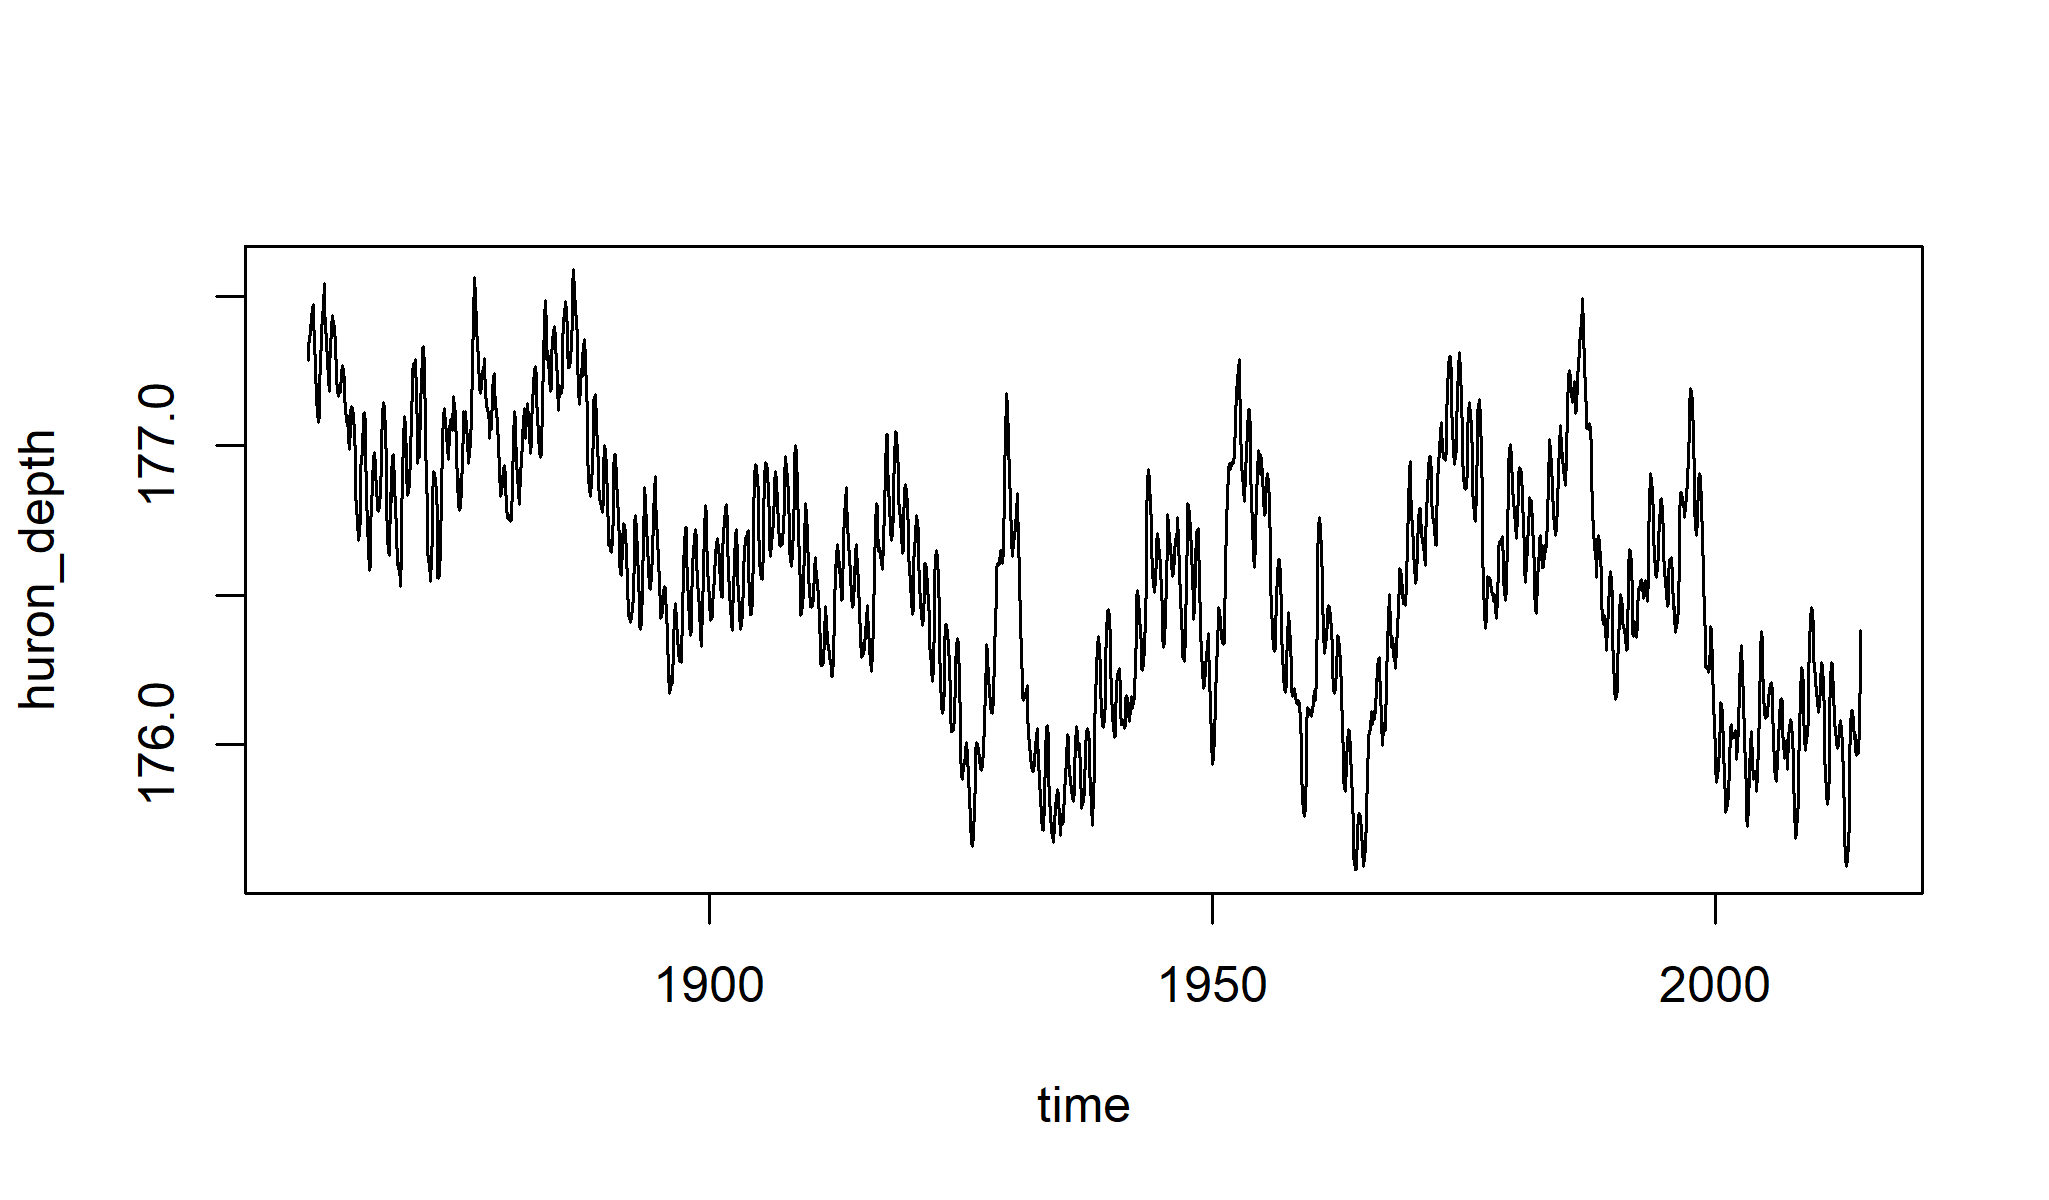
\includegraphics{figure/intro-plot_data-1} \end{center}

\begin{itemize}
\tightlist
\item
  Now, we get to fit a model. Based on our previous analysis, we'll go
  with AR(1) for the annual polynomial. Let's try ARMA(1,1) for the
  monthly part. In other words, we seek to fit the model
  \[ (1-\AR_1 B^{12})(1-\ar_1 B) Y_n = (1+\ma_1 B)\epsilon_n.\]
  \todo[inline]{Left-most part, i.e. $(1-\Phi_1 B^{12})$ is the AR(1) annual polynomial - there's no corresponding annual poly on right b/c AR(1) doesn't include a moving-average (MA) term.}
  \todo[inline]{Poly $(1-\phi_1 B)$, along with poly on right, i.e. $(1 + \psi_1B)$, make up the ARMA(1,1) polynomials for the monthly part of the model. (See notes4 The General ARMA Model)}
\end{itemize}

\begin{Shaded}
\begin{Highlighting}[]
\NormalTok{huron_sarma11x10 <-}\StringTok{ }\KeywordTok{arima}\NormalTok{(huron_depth,}
   \DataTypeTok{order=}\KeywordTok{c}\NormalTok{(}\DecValTok{1}\NormalTok{,}\DecValTok{0}\NormalTok{,}\DecValTok{1}\NormalTok{),}
   \DataTypeTok{seasonal=}\KeywordTok{list}\NormalTok{(}\DataTypeTok{order=}\KeywordTok{c}\NormalTok{(}\DecValTok{1}\NormalTok{,}\DecValTok{0}\NormalTok{,}\DecValTok{0}\NormalTok{),}\DataTypeTok{period=}\DecValTok{12}\NormalTok{)}
\NormalTok{)}
\NormalTok{huron_sarma11x10}
\end{Highlighting}
\end{Shaded}

\todo[inline]{In code above, order args are p, diff, q (no difference here), still stationary model.}

\begin{verbatim}
## 
## Call:
## arima(x = huron_depth, order = c(1, 0, 1), seasonal = list(order = c(1, 0, 0), 
##     period = 12))
## 
## Coefficients:
##          ar1     ma1    sar1  intercept
##       0.9641  0.3782  0.5104   176.5714
## s.e.  0.0063  0.0203  0.0218     0.0909
## 
## sigma^2 estimated as 0.002592:  log likelihood = 2884.36,  aic = -5758.72
\end{verbatim}

\begin{itemize}
\item
  Residual analysis is similar to what we've seen for non-seasonal ARMA
  models.
\item
  We look for residual correlations at lags corresonding to multiples of
  the period (here, 12, 24, 36, \ldots{}) for misspecified annual
  dependence.
\end{itemize}

\begin{Shaded}
\begin{Highlighting}[]
\KeywordTok{acf}\NormalTok{(}\KeywordTok{resid}\NormalTok{(huron_sarma11x10))}
\end{Highlighting}
\end{Shaded}

\begin{center}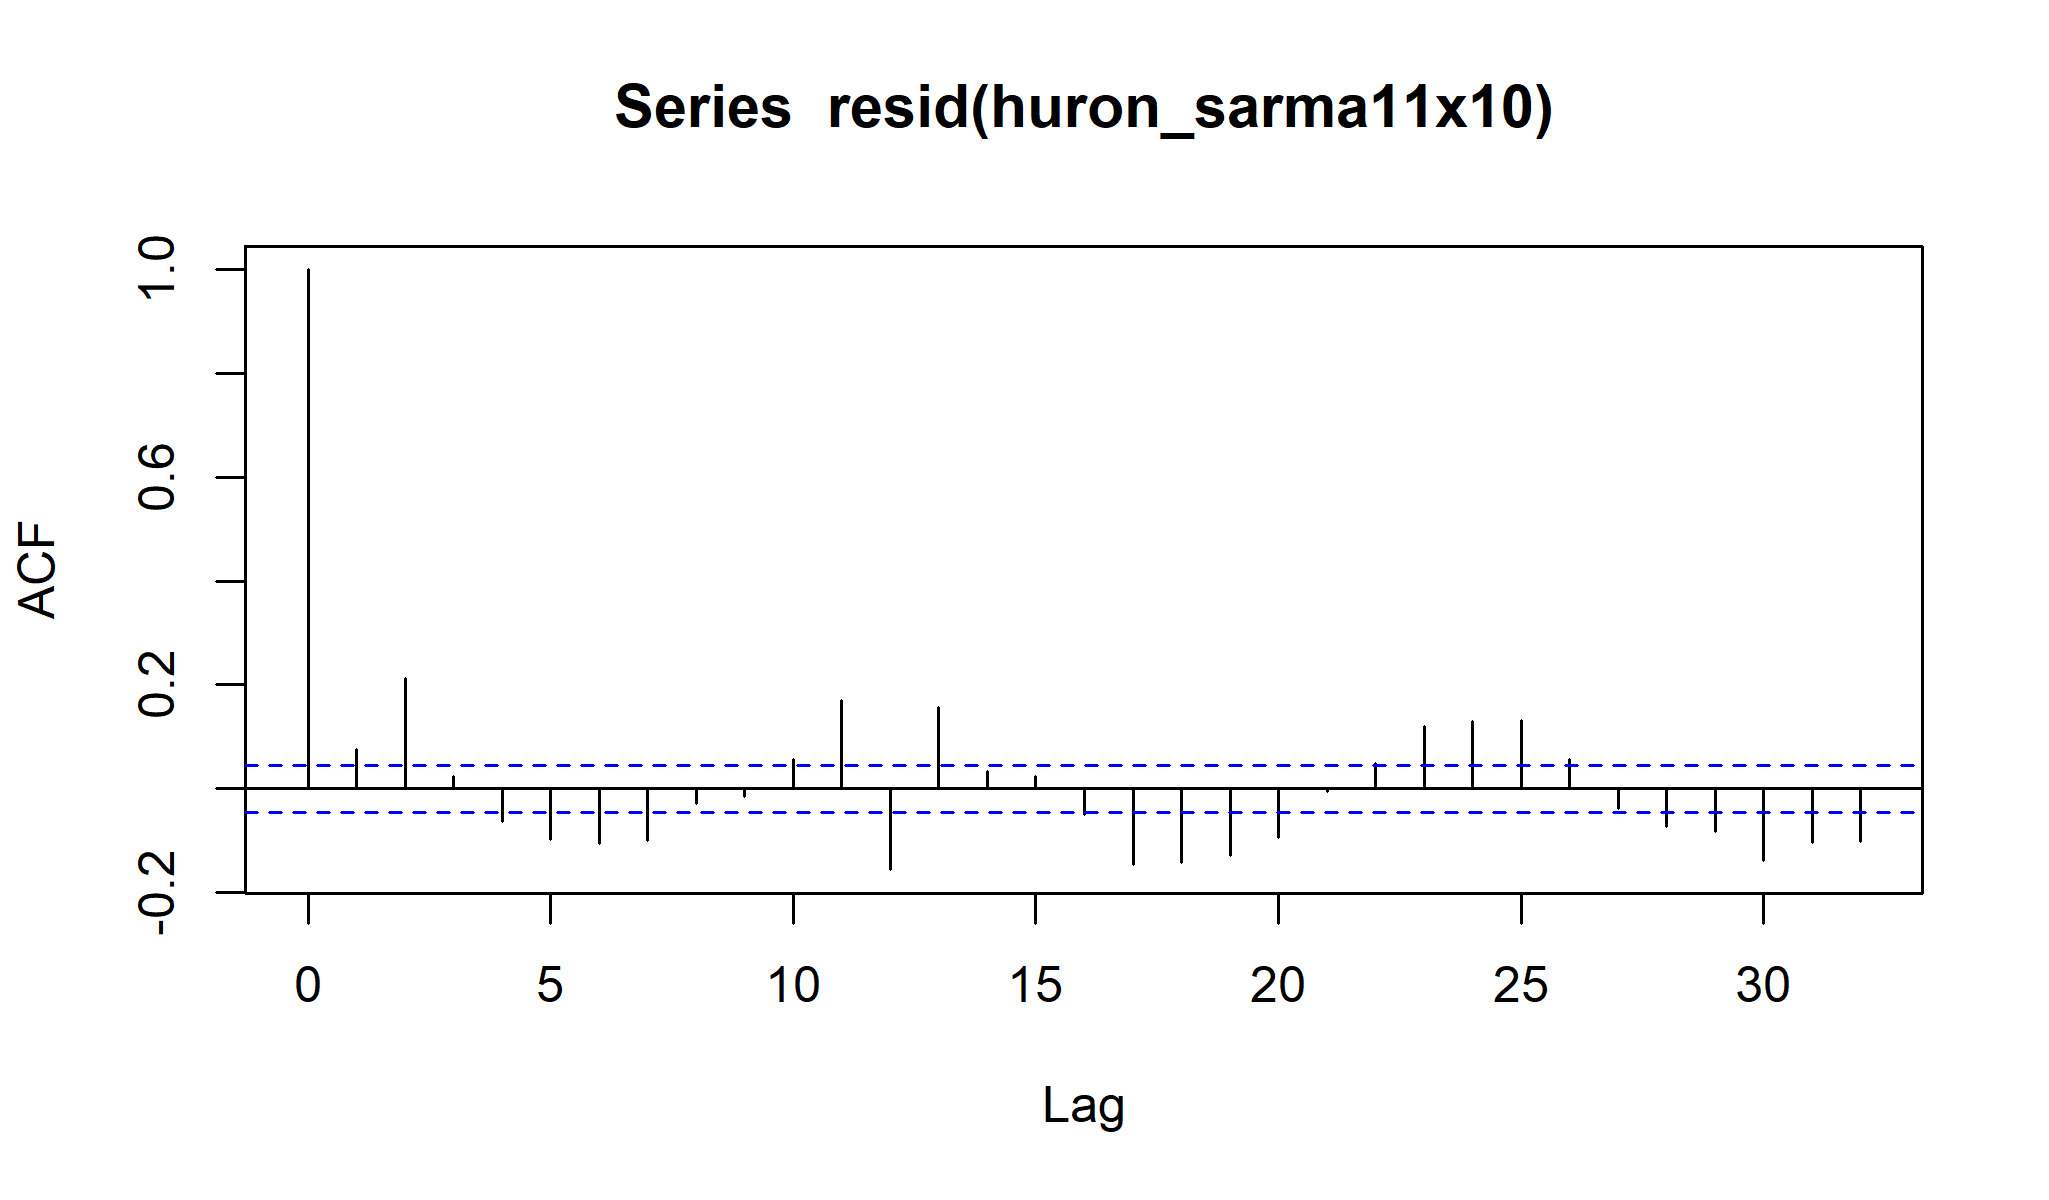
\includegraphics{figure/intro-residuals-1} \end{center}

\begin{center}\rule{0.5\linewidth}{\linethickness}\end{center}

\begin{center}\rule{0.5\linewidth}{\linethickness}\end{center}

\subsubsection{Question: What do you conclude from this residual
analysis? What would you do
next?}\label{question-what-do-you-conclude-from-this-residual-analysis-what-would-you-do-next}

\todo[inline]{The current model isn't capturing all the dependence in the data. Maybe add AR(2) term to fit the lag residual correlation. (Adding more AR terms could be good b/c we see an oscillatory behavior in the residual ACF)}

\begin{center}\rule{0.5\linewidth}{\linethickness}\end{center}

\begin{center}\rule{0.5\linewidth}{\linethickness}\end{center}

\subsection{ARMA models for differenced
data}\label{arma-models-for-differenced-data}

\begin{itemize}
\item
  \hl{Applying a difference operation to the data can make it look more
  stationary} and therefore more appropriate for ARMA modeling.
\item
  This can be viewed as a \hl{\textbf{transformation to stationarity}}
\item
  We can transform the data \(\data{y_{1:N}}\) to \(\data{z_{2:N}}\)
  \[ \data{z_n} = \Delta \data{y_n} = \data{y_n}-\data{y_{n-1}}.\]
\item
  Then, an ARMA(p,q) model \(Z_{2:N}\) for the differenced data
  \(\data{z_{2:N}}\) is called an \hl{\textbf{integrated autoregressive
  moving average}} model for \(\data{y_{1:N}}\) and is written as
  ARIMA(p,1,q).
\item
  Formally, the ARIMA(p,d,q) model with \hl{intercept $\mu$} for
  \(Y_{1:N}\) is
  \[[S4] \eqspace \ar(B)\big( (1-B)^d Y_n-\mu) = \ma(B) \epsilon_n,\]
  where \(\{\epsilon_n\}\) is a white noise process; \(\ar(x)\) and
  \(\ma(x)\) are the ARMA polynomials defined previously.
\item
  It is \hl{unusual to fit an ARIMA model with $d>1$.}
\item
  We see that an ARIMA(p,1,q) model is almost a special case of an
  ARMA(p+1,q) model with a \textbf{unit root} to the AR(p+1) polynomial.
\end{itemize}

\begin{center}\rule{0.5\linewidth}{\linethickness}\end{center}

\begin{center}\rule{0.5\linewidth}{\linethickness}\end{center}

\subsubsection{\texorpdfstring{Question: why ``almost'' not ``exactly''
in the previous
statement?}{Question: why almost not exactly in the previous statement?}}\label{question-why-almost-not-exactly-in-the-previous-statement}

\todo[inline]{This is almost true b/c it treates the mean slightly differently.}

\begin{center}\rule{0.5\linewidth}{\linethickness}\end{center}

\begin{center}\rule{0.5\linewidth}{\linethickness}\end{center}

\subsubsection{Why fit an ARIMA model?}\label{why-fit-an-arima-model}

\begin{itemize}
\tightlist
\item
  There are two reasons to fit an ARIMA(p,1,q) model
\end{itemize}

\begin{enumerate}
\def\labelenumi{\arabic{enumi}.}
\item
  You may really think that modeling the differences is a natural
  approach for your data. The S\&P 500 stock market index analysis in
  \href{../03/notes03.html\#a-random-walk-model}{Section 3.5} is an
  example of this, as long as you remember to first apply a logarithmic
  transform to the data.
\item
  \hl{Differencing often makes data look ``more stationary''} and perhaps it
  will then look stationary enough to justify applying the ARMA
  machinery.
\end{enumerate}

\begin{itemize}
\item
  We should be cautious about this second reason. It can lead to poor
  model specifications and hence poor forecasts or other conclusions.
\item
  The second reason was more compelling in the 1970s and 1980s. With
  limited computing power and the existence of computationally
  convenient (but statistically inefficient) method-of-moments
  algorithms for ARMA, it made sense to force as many data analyses as
  possible into the ARMA framework.
\item
  ARIMA analysis is relatively simple to do. It has been a foundational
  component of time series analysis since the publication of the
  influential book ``Time Series Analysis'' by Box and Jenkins (1st
  edition, 1970) which developed and popularized ARIMA modeling. A
  practical approach is:
\end{itemize}

\begin{enumerate}
\def\labelenumi{\arabic{enumi}.}
\item
  Do a competent ARIMA analysis.
\item
  Identify potential limitations in this analysis and remedy them using
  more advanced methods.
\item
  Assess whether you have in fact learned anything from (2) that goes
  beyond (1).
\end{enumerate}

\begin{center}\rule{0.5\linewidth}{\linethickness}\end{center}

\begin{center}\rule{0.5\linewidth}{\linethickness}\end{center}

\subsubsection{Question: What is the trend of the ARIMA(p,1,q)
model?}\label{question-what-is-the-trend-of-the-arimap1q-model}

\begin{itemize}
\tightlist
\item
  Hint: recall that the ARIMA(p,1,q) model specification for \(Y_{1:N}\)
  implies that \(Z_n = (1-B)Y_n\) is a stationary, causal, invertible
  ARMA(p,q) process with mean \(\mu\). Now take expectations of both
  sides of the difference equation.
\end{itemize}

\todo[inline]{$\EE[(1-B)Y_n] = \mu\implies (1-B)\EE(Y_n)=\mu\implies \EE(Y_n)-\EE(Y{n-1})=\mu\implies \EE(Y_n) = \mu + \EE(Y_{n-1})$. Thus, $\EE(Y_n) = n\mu + constant$,  i.e. the difference $z_n$ has constant mean $\mu$, but $Y_n$ has mean increasing/decreasing with $n$ (linear mean, non-stationary). }


\begin{center}\rule{0.5\linewidth}{\linethickness}\end{center}

\begin{center}\rule{0.5\linewidth}{\linethickness}\end{center}

\subsubsection{\texorpdfstring{Question: What is the trend of the
ARIMA(p,d,q) model, for general
\(d\)?}{Question: What is the trend of the ARIMA(p,d,q) model, for general d?}}\label{question-what-is-the-trend-of-the-arimapdq-model-for-general-d}

\todo[inline]{Note. $d=2\implies$ quadratic trend, $d=3\implies$ cubic trend, etc.}

\begin{center}\rule{0.5\linewidth}{\linethickness}\end{center}

\begin{center}\rule{0.5\linewidth}{\linethickness}\end{center}

\subsection{\texorpdfstring{The SARIMA\((p,d,q)\times(P,D,Q)\)
model}{The SARIMA(p,d,q)\textbackslash{}times(P,D,Q) model}}\label{the-sarimapdqtimespdq-model}

\begin{itemize}
\item
  Combining integration of ARMA models with seasonality, we can write a
  general SARIMA\((p,d,q)\times(P,D,Q)_{12}\) model for \hl{nonstationary
  monthly data}, given by
  \[[S5] \eqspace \ar(B)\AR(B^{12}) \big((1-B)^d(1-B^{12})^D Y_n-\mu)= \ma(B)\MA(B^{12}) \epsilon_n,\]
  where \(\{\epsilon_n\}\) is a white noise process, the intercept
  \(\mu\) is the mean of the differenced process
  \(\{(1-B)^d(1-B^{12})^D Y_n\}\), and we have ARMA polynomials
  \(\ar(x)\), \(\AR(x)\), \(\ma(x)\), \(\MA(x)\) as in model {[}S1{]}.
\item
  The SARIMA\((0,1,1)\times(0,1,1)_{12}\) model has often been \hl{used for
  forecasting monthly time series in economics and business}. It is
  sometimes called the \textbf{airline model} after a data analysis by
  Box and Jenkins (1970).
\end{itemize}

\begin{center}\rule{0.5\linewidth}{\linethickness}\end{center}

\begin{center}\rule{0.5\linewidth}{\linethickness}\end{center}

\subsection{Modeling trend with ARMA
noise.}\label{modeling-trend-with-arma-noise.}

\begin{itemize}
\item
  A general \hl{\textbf{signal plus noise} model} is
  \[[S6] \eqspace   Y_n = \mu_n + \eta_n,\] where \(\{\eta_n\}\) is a
  stationary, mean zero stochastic process, and \(\mu_n\) is the mean
  function.
\item
  If, in addition, \(\{\eta_n\}\) is uncorrelated, then we have a
  \textbf{signal plus white noise} model. \hl{The usual linear trend
  regression model fitted by least squares in
  Section 2.4 corresponds to a signal plus white noise model.}
\item
  We can say \textbf{signal plus colored noise} if we wish to emphasize
  that we're not assuming white noise.
\item
  Here, \textbf{signal} and \textbf{trend} are used interchangeably. In
  other words, we are assuming a deterministic signal.
\item
  At this point, it is natural for us to consider a signal plus
  ARMA(p,q) noise model, where \(\{\eta_n\}\) is a stationary, causal,
  invertible ARMA(p,q) process with mean zero.
\item
  As well as the \(p+q+1\) parameters in the ARMA(p,q) model, there \hl{will
  usually be unknown parameters in the mean function}. In this case, we
  can write \[ \mu_n = \mu_n(\beta)\] where \hl{$\beta$ is a vector of
  unknown paramters, $\beta\in\R^K$.}
\item
  We write \(\theta\) for a vector of all the \(p+q+1+K\) parameters, so
  \[\theta = (\ar_{1:p},\ma_{1:q},\sigma^2,\beta).\]
\end{itemize}

\begin{center}\rule{0.5\linewidth}{\linethickness}\end{center}

\begin{center}\rule{0.5\linewidth}{\linethickness}\end{center}

\subsubsection{Linear regression with ARMA
errors}\label{linear-regression-with-arma-errors}

\begin{itemize}
\item
  When the trend function has a linear specification,
  \[\mu_n = \sum_{k=1}^K Z_{n,k}\beta_k,\]
   the \textbf{signal plus ARMA
  noise} model is known as \hl{\textbf{linear regression with ARMA errors}}.
\todo[inline]{Here, $\mu_n$ encodes the trend for the data.}
\item
  Writing \(Y\) for a column vector of \(Y_{1:N}\), \(\mu\) for a column
  vector of \(\mu_{1:N}\), \(\eta\) for a column vector of
  \(\eta_{1:N}\), and \(Z\) for the \(N\times K\) matrix with \((n,k)\)
  entry \(Z_{n,k}\), we have a \hl{general linear regression model with
  correlated ARMA errors}, \[ Y = Z\beta + \eta.\]
\item
  Maximum likelihood estimation of
  \(\theta = (\ar_{1:p},\ma_{1:q},\sigma^2,\beta)\) is a nonlinear
  optimization problem. Fortunately, \texttt{arima} in R can do it for
  us, though as usual we should look out for signs of numerical
  problems.
\item
  \hl{Data analysis for a linear regression with ARMA errors model}, using
  the framework of likelihood-based inference, is therefore procedurally
  similar to fitting an ARMA model.
\item
  This is a powerful technique, since the covariate matrix \(Z\) can
  include other time series. We can \hl{evaluate associations between
  different time series}. With appropriate care (since
  \textbf{association is not causation}) we can draw inferences about
  mechanistic relationships between dynamic processes.
\end{itemize}

\begin{center}\rule{0.5\linewidth}{\linethickness}\end{center}

\begin{center}\rule{0.5\linewidth}{\linethickness}\end{center}

\subsubsection{Example: Looking for evidence of systematic trend in the
depth of Lake
Huron}\label{example-looking-for-evidence-of-systematic-trend-in-the-depth-of-lake-huron}

\begin{itemize}
\tightlist
\item
  Let's restrict ourselves to annual data, say the January depth.
\end{itemize}

\begin{Shaded}
\begin{Highlighting}[]
\NormalTok{monthly_dat <-}\StringTok{ }\KeywordTok{subset}\NormalTok{(dat, month}\OperatorTok{==}\DecValTok{1}\NormalTok{)}
\NormalTok{huron <-}\StringTok{ }\NormalTok{monthly_dat}\OperatorTok{$}\NormalTok{Average}
\NormalTok{year <-}\StringTok{ }\NormalTok{monthly_dat}\OperatorTok{$}\NormalTok{year}
\KeywordTok{plot}\NormalTok{(}\DataTypeTok{x=}\NormalTok{year,}\DataTypeTok{y=}\NormalTok{huron,}\DataTypeTok{type=}\StringTok{"l"}\NormalTok{)}
\end{Highlighting}
\end{Shaded}

\begin{center}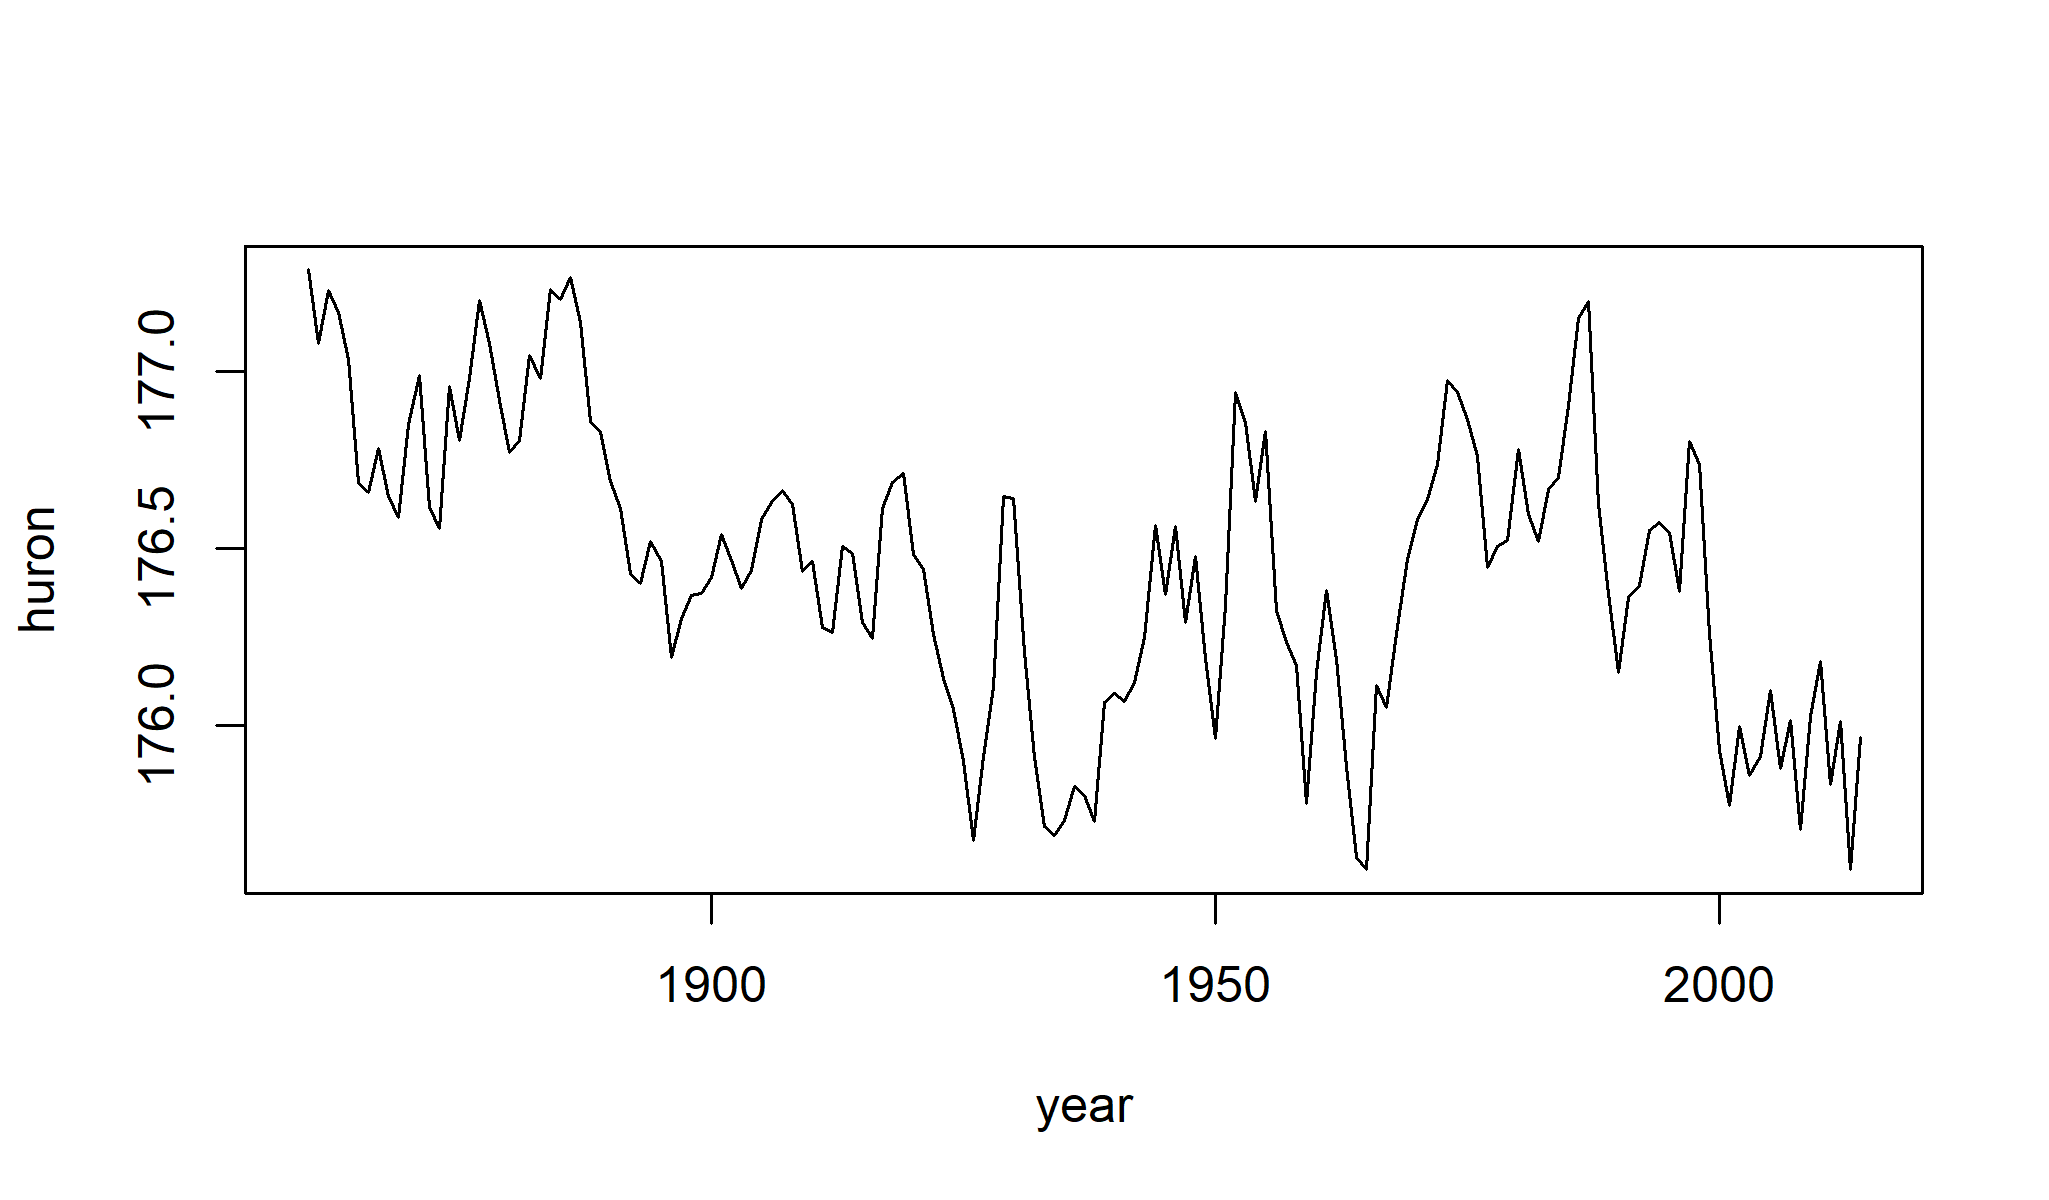
\includegraphics{figure/intro-data_subset-1} \end{center}

\begin{itemize}
\item
  Visually, there seems some evidence for a decreasing trend, but there
  are also considerable fluctuations.
\item
  Let's test for a trend, using a \hl{regression model with Gaussian AR(1)
  errors}. We have previously found that this is a reasonable model for
  these data.
\item
  First, let's fit a null model.
\end{itemize}

\begin{Shaded}
\begin{Highlighting}[]
\NormalTok{fit0 <-}\StringTok{ }\KeywordTok{arima}\NormalTok{(huron,}\DataTypeTok{order=}\KeywordTok{c}\NormalTok{(}\DecValTok{1}\NormalTok{,}\DecValTok{0}\NormalTok{,}\DecValTok{0}\NormalTok{))}
\NormalTok{fit0}
\end{Highlighting}
\end{Shaded}

\begin{verbatim}
## 
## Call:
## arima(x = huron, order = c(1, 0, 0))
## 
## Coefficients:
##          ar1  intercept
##       0.8694   176.4588
## s.e.  0.0407     0.1234
## 
## sigma^2 estimated as 0.04368:  log likelihood = 22,  aic = -38
\end{verbatim}

\begin{itemize}
\tightlist
\item
  Now, we can compare with a linear trend model.
\end{itemize}

\begin{Shaded}
\begin{Highlighting}[]
\NormalTok{fit1 <-}\StringTok{ }\KeywordTok{arima}\NormalTok{(huron,}\DataTypeTok{order=}\KeywordTok{c}\NormalTok{(}\DecValTok{1}\NormalTok{,}\DecValTok{0}\NormalTok{,}\DecValTok{0}\NormalTok{),}\DataTypeTok{xreg=}\NormalTok{year)}
\NormalTok{fit1}
\end{Highlighting}
\end{Shaded}

\begin{verbatim}
## 
## Call:
## arima(x = huron, order = c(1, 0, 0), xreg = year)
## 
## Coefficients:
##          ar1  intercept     year
##       0.8240   186.0146  -0.0049
## s.e.  0.0451     3.7417   0.0019
## 
## sigma^2 estimated as 0.0423:  log likelihood = 24.62,  aic = -41.25
\end{verbatim}
\todo[inline]{In code above, $\beta$ is coefficient associated with year (mean function or trend only a function of year)}
\begin{itemize}
\tightlist
\item
  To talk formally about these results, we'd better write down a model
  and some hypotheses. Writing the data as \(\data{y_{1:N}}\), collected
  at years \(t_{1:N}\), the model we have fitted is
  \[ (1-\ar_1 B)(Y_n - \mu - \beta t_n) = \epsilon_n,\] 
  \todo[inline]{Here, our regression model is $Y_n = \mu + \beta t_n + e_n=\mu_n + e_n$ where $e_n$ are the errors of the regression model. Then $(1-\phi_1B)e_n = \epsilon_n$ is an AR(1) model for the errors $e_n = Y_n - \mu-\beta t_n$.}
  where
  \(\{\epsilon_n\}\) is Gaussian white noise with variance \(\sigma^2\).
  Our null model is \[ H^{\langle 0\rangle}: \beta=0,\] and our
  alternative hypothesis is \[ H^{\langle 1\rangle}: \beta\neq 0.\]
\end{itemize}

\begin{center}\rule{0.5\linewidth}{\linethickness}\end{center}

\begin{center}\rule{0.5\linewidth}{\linethickness}\end{center}

\subsubsection{\texorpdfstring{Question: How do we test
\(H^{\langle 0\rangle}\) against
\(H^{\langle 1\rangle}\)?}{Question: How do we test H\^{}\{\textbackslash{}langle 0\textbackslash{}rangle\} against H\^{}\{\textbackslash{}langle 1\textbackslash{}rangle\}?}}\label{question-how-do-we-test-hlangle-0rangle-against-hlangle-1rangle}

\begin{itemize}
\item
  Construct two different tests using the R output above.
  \todo[inline]{1) t-test for $\beta$ (Fiher info CI), 2) likelihood ratio test (profile CI). Here, $\Delta loglik = 2.62$. The LRT compares $2\Delta loglik$ with $\chi^2$. We obtain a p-value of $1-pchisq(5.24,1) = 0.02$. Thus, we reject the null model.}
\item
  Which test do you prefer, and why?
\item
  How would you check whether your preferred test is indeed better?
\end{itemize}

\begin{center}\rule{0.5\linewidth}{\linethickness}\end{center}

\begin{center}\rule{0.5\linewidth}{\linethickness}\end{center}

\subsubsection{Question: What other supplementary analysis could you do
to strengthen your
conclusions?}\label{question-what-other-supplementary-analysis-could-you-do-to-strengthen-your-conclusions}
\todo[inline]{simulation under the null hypothesis}
\begin{center}\rule{0.5\linewidth}{\linethickness}\end{center}

\begin{center}\rule{0.5\linewidth}{\linethickness}\end{center}


\end{document}
